\chapter{Clustering Patient Visits}
\label{chapter:clustering}

As described in Chapter~\ref{chapter:intro}, all patients data is retrieved from the database directly. These data only records information about patient visits, but without any manual labels indicating which visits are abnormal. Due to lack of labels, unsupervised learning algorithms should be adopted. Clustering is a collection of unsupervised methods, which identifies groups of data points according to a defined similarity metric, such that objects in the same group posses higher similarities compared to objects in other groups. The clustering process does not rely on labels but the choice of similarity metrics. Variations in similarity metrics lead to different clustering methods.

Applying clustering methods in anomaly detection tasks has been studied numerously~\cite{he2003discovering}
. This chapter introduces two typical methods, K-Means~\cite{lloyd1982least} and DBSCAN~\cite{ester1996density}. Problem formulation, solutions, and potential issues are formally described using elaborated notations in following sections. However, analysis on the performance and constraints of these two methods are postponed to Chapter~\ref{chapter:experiments}, which reveals their practicality and infeasibility in the previously described anomaly detection problem.

\section{K-Means}
\label{sec:k-means}

K-Means~\cite{lloyd1982least} is one of the simplest unsupervised algorithm which solves clustering problem. Despite its simplicity, K-Means has gained success in various situations, including anomaly detection~\cite{campello2015hierarchical}\cite{he2003discovering}, image segmentation and compression~\cite{forsyth2002computer}. K-Means is also frequently used as pre-processing for more complicated algorithms. The method can be formally defined as follow: Given a data set $\{\mathbf{x}_1, ... , \mathbf{x}_N\}$ consisting of $N$ observations in $D$-dimensional space, the object is to partition the data into $K$ groups, by defining a set of $K$ centres $\{\boldsymbol{\mu}_1, ... , \boldsymbol{\mu}_k\}$ in the same space, and assigning each observation to exactly one center point. Each center point represents a prototype associated with the $k^{th}$ cluster.

The assignments can be represented using 1-of-$K$ schema. Then, for each data point $x_n$, a corresponding  $K$-dimensional variable consisting of $K$ binary elements $r_{nk} \in \{0, 1\}$ is introduced. Among these $r_{nk}$, exactly one of them equals 1, which means $\mathbf{x}_{n}$ belongs to the $k^{th}$ cluster. Using this notation, evaluation of the clustering quality can be defined using the object function as follow:
\begin{equation}	
	\label{eq:kmeansobj}
	J = \sum_{n=1}^{N}\sum_{k=1}^{K}r_{nk}D(\mathbf{x}_{N} - \boldsymbol{\mu}_{k})
\end{equation}
where $D$ is a dissimilarity metric. Common choice of the metric is $\mathit{l}_1$-norm or $\mathit{l}_2$-norm. Mahalanobis distance is also adopted while considering the covariances between the $K$-dimensions~\cite{davis1986statistics}. In the following context, $\mathit{l}_2$-norm is adopted for discussion. 
 Intuitively, this function can be considered as the distance summation of each point to its corresponding cluster prototype $\boldsymbol{\mu}_k$. The K-Means aims at finding a set of $\boldsymbol{\mu}_k$ which minimizes the object function. Finding the optimal solution for the above object function proves to be NP-Hard~\cite{aloise2009np}. However, employing heuristic algorithms enables finding converged local optimal solutions. Section~\ref{subsec:EM} describes one iterative algorithm, EM. Section~\ref{subsec:KMeansIssues} explores common issues related to K-Means and remedies.
\subsection{EM Algorithm in K-Means}
\label{subsec:EM}

EM algorithm~\cite{dempster1977maximum} is an iterative algorithm to find local maximum. Each iteration consists of two phases, Expectation and Maximization, which corresponds to minimize the objective function $J$ with respect to $r_{nk}$ and $\boldsymbol{\mu}_{k}$ respectively. In the E(expectation) step, the algorithm minimize $J$ with respect to $r_{nk}$, while keeping the $\boldsymbol{\mu}_{k}$ fixed. Then in the following M(maximization) step, the algorithm minimizes $J$ with respect to $\boldsymbol{\mu}_{k}$, while keeping $r_{nk}$ fixed. 

Considering the optimization in E step, a critical observation of \eqref{eq:kmeansobj} is that \(\mathbf{r}_n\)'s are independent of each other. Thus, optimization on \(\mathbf{r}_n\)'s can be done separately for each \(n\). The solution is simply setting the \(r_{nk}\) corresponding to the minimum \(\| \mathbf{x}_n - \boldsymbol{\mu}_k \|^2\) to 1.  Intuitively, the algorithm assigns \(\mathbf{x}_n\) to the closest cluster center. Formally, the solution can be written as
\begin{equation}
 r_{nk} =
    \begin{cases}
        1   & \quad \text{if } k = \operatorname{arg\,min}_j \parallel \mathbf{x}_{n} - \mathbf{\mu}_{j} {\parallel}^2 \\
        0   & \quad \text{otherwise}
    \end{cases}
\end{equation}

In the following M step, the above determined \(r_{nk}\) is clamped. Then, \(\boldsymbol{\mu}_k\) appears only in a quadratic term in \(J\). Setting derivatives of \(J\) with respect to \(\boldsymbol{\mu}_k\) to zero, solution formula for \(\boldsymbol{\mu}_k\) can be expressed in following closed form
\begin{equation}
	\label{eq:muupdate}
	\boldsymbol{\mu}_{k} = \frac{\sum_n r_{nk}\mathbf{x}_n}{\sum_n r_{nk}}
\end{equation}
This step can be considered as recomputing the cluster prototype by setting \(\boldsymbol{\mu}_k\) to the mean of all points assigned to that cluster. 

EM keeps executing these two steps alternatively, until a convergence happens or until number of iterations exceeded a predefined value. Since in each phase, one variable is fixed and updating another variable minimizes the cost function \(J\), convergence is guaranteed. Formal proof on convergence has been studied by MacQueen~\cite{macqueen1967some}.

The algorithm is illustrated using dataset generated independently from three Gaussian distributions in Figure~\ref{fig:EM4KMeans}. In this demonstration, the algorithm takes \(K\) = 3, which is the correct number of components. Before running the first iteration, initialized \(\boldsymbol{\mu}_k\) is required. This initialization is done by choosing three objects from the data set randomly.

\begin{figure}
	\begin{center}
		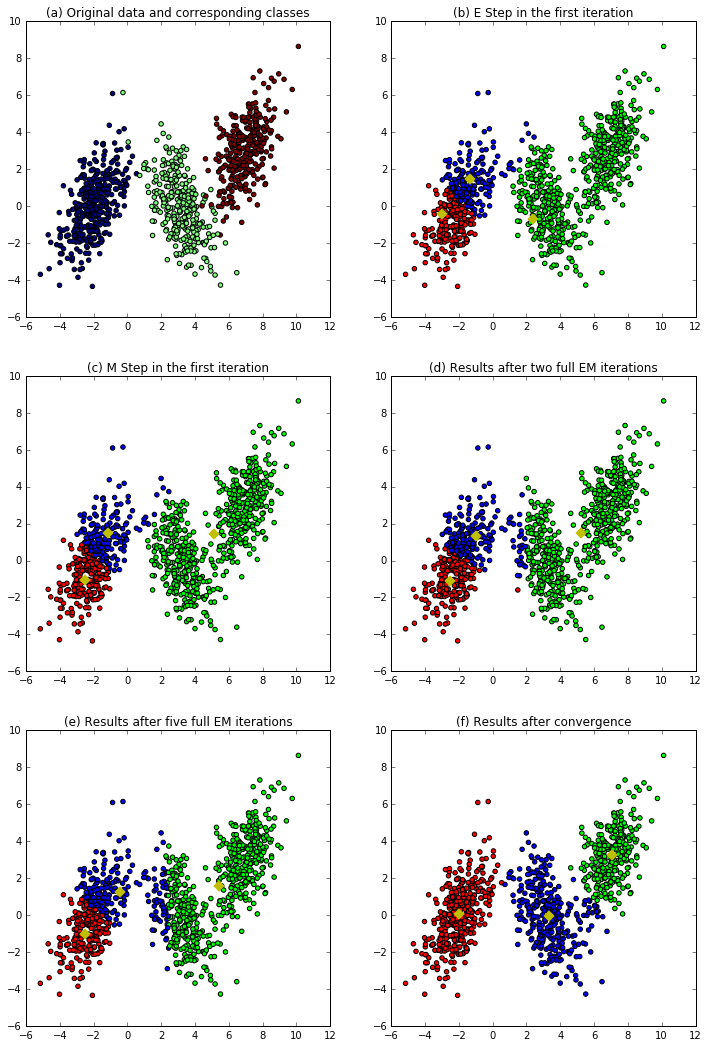
\includegraphics[width=\textwidth]{images/EM4KMeans.png}
		\caption{Illustration of EM algorithm on K-Means using data generated independently from three Gaussian distribution. (a) Original data and corresponding classes. Classes are denoted in different colors. (b) Assignments of each data after the first E step. The yellow diamonds represent the initialized \(\boldsymbol{\mu}_k\). (c) Updated \(\boldsymbol{\mu}_k\) after the M step in the first iteration. (d)-(f) Clustering results after several successive full EM iterations until convergence is met.}
		\label{fig:EM4KMeans}
	\end{center}
\end{figure}

\subsection{Issues in K-Means}
\label{subsec:KMeansIssues}
Despite the simplicity of K-Means, several underlying issues exists. The first potential is that, how to choose the value for \(K\). In the above illustration, \(K\) was set to 3 which is the correct number of components. However, if \(K\) wasn't set to the correct value, unsatisfied clustering may be generated. Example of this issue is shown in Figure~\ref{fig:KMeansIssue}(a)-(c). To solve this problem, one practical way is drawing graph of the cost function versus value of \(K\), as shown in Figure~\ref{fig:KMeansIssue}(d). Intuitively, when \(K\) is under smaller than the true number of clusters, increasing \(K\) will lead to a huge drop of cost function value. However, when \(K\) has reached or exceeded the correct value, increasing \(K\) leads only small cost function value drop. Thus, number of clusters corresponding to the `elbow' point can be considered as the real number of clusters.

\begin{figure}
	\begin{center}
		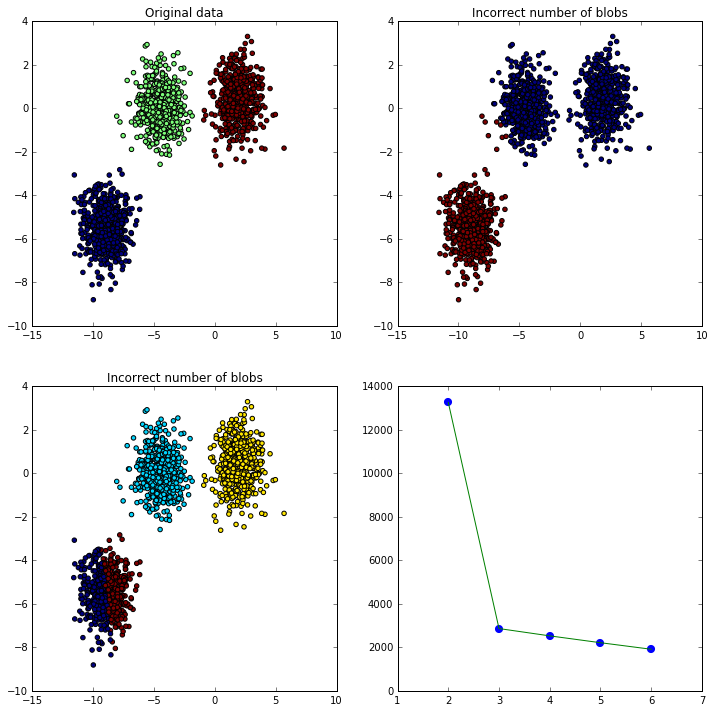
\includegraphics[width=\textwidth]{images/KMeansIncorrectNumber.png}
		\caption{Issues of K-Means incurred by choosing inappropriate value for \(K\)}
		\label{fig:KMeansIssue}
	\end{center}
\end{figure}

Another issues of K-Means relates to the initialization of \(\boldsymbol{\mu}_k\). Since EM finds only local optimal solutions, a poor initialization could lead to worse clustering result. To avoid this problem, it is practical to run K-Means for several times and choose the best result according to the value of the cost function.

One more critical issue of K-Means lies in the choice of similarity metric. As mentioned at the beginning of this chapter, variations in similarity metric leads to different clustering methods. Choosing \(l\)-2 norm is convenient in terms of computation, but this choice limits the type of data variables to certain types. Using \(l\)-2 norm on categorical data is inappropriate since no ordering of categorical values exists. Also, this makes computing the mean value a hard problem. To use K-Means on other data types, the similarity metric should be elaborately designed. 

Besides, K-Means tends to form clusters into a convex space. As shown in Figure~\ref{fig:EM4KMeans}(b)-(e), the boundary between two different clusters forms a line lying at the midway and is perpendicular to the line connecting two cluster prototypes. However, a cluster is not necessary to be convext. This also limits the application of K-Means.

Finally, K-Means is also sensitive to noises. As shown in formula \ref{eq:muupdate}, updating \(\boldsymbol{\mu}_k\) involves computing the mean of all data points assigned to that cluster. When noise objects with large deviation from other points in this cluster exist, update of \(\boldsymbol{\mu}_k\) will be strongly affected. 

\section{Density Based Clustering Methods}
This section explores another type of clustering method which forms cluster from the view of density aspect. \textbf{D}ensity-\textbf{B}ased \textbf{S}patial \textbf{C}lustering of \textbf{A}pplications with \textbf{N}oise (DBSCAN)~\cite{ester1996density} considers to be one of the most successful method from this category~\cite{2014timeaward}. Compared to K-Means, DBSCAN posseses following advantages: 1).\ DBSCAN can detect clusters of arbitrary shape. 2).\ DBSCAN can determine the number of clusters automatically. 3).\ DBSCAN is robust to noises. 

The following of this chapter is organized as follows. Section~\ref{subsec:DBSCANDFS} compares and reveals the relation of DBSCAN to a basic graph traversal algorithm \textbf{D}epth \textbf{F}irst \textbf{S}earch(DFS). This section will introduce the critical concept used by DBSCAN which differentiate it with DFS. Section ~\ref{subsec:DBSCANnotion} describe this concept in more details. Section~\ref{subsec:DBSCANalgorithm} compares DBSCAN and K-Means, and discusses practical issues of DBSCAN.

\subsection{DBSCAN and DFS}
\label{subsec:DBSCANDFS}
Before introducing DBSCAN, it would be helpful to review a basic graph traversal algorithm, DFS, which is an algorithm which traverses or visits a graph. In the discussion of this context, the whole process is divided into two procedures \proc{DFS} and \proc{DFS-Visit}. A typical recursive implementation is described as follow. 

\begin{codebox}
\Procname{$\proc{DFS}(G)$}
\li \For each vertex $u \in G$
\li		\Do
			$\attrib{u}{visited} \gets \const{false}$
	\End
\li	\For each vertex $u \in G$
\li		\Do
		\If \(\attrib{u}{visited} \isequal \const{false}\)
\li			\Then
				$\proc{DFS-Visit}(G, u)$
		\End
	\End
\end{codebox}

\begin{codebox}
\Procname{$\proc{DFS-Visit}(G, u)$}
\li	$\attrib{u}{visited} \gets \const{true}$
\li	\For each vertex $v \in \attrib{G}{Adj}[u]$
\li	\Do
		\If	$\attrib{v}{visited} \isequal \const{false} $
\li			\Then
				$\proc{DFS-Visit}(G, v)$
		\End
	\End
\end{codebox}

The first two lines in \proc{DFS} initializes the algorithm by setting all nodes to be unvisited. Then, the algorithm traverse vertices in the graph. Once an unvisited node is found, \proc{DFS-Visit} is called. In the procedure \proc{DFS-Visit}, the given node $u$ is labelled as visited. If an unvisited child $v$ of $u$ is found, this procedure goes one layer deeper by calling another \proc{DFS-Visit} on $v$. After finishing $\proc{DFS-Visit}(G, u)$, the algorithm backtrack to visit other unvisited children of $u$, which are siblings of $v$.

Assume \proc{DFS} executes on an undirected graph. Each call of $\proc{DFS-Visit}$ on an unvisited node $u$ explores $u$ and all nodes reachable to it. These nodes form a component which disconnects with other components by other runs of $\proc{DFS-Visit}$. Thus, each component can be considered as a cluster. The criterion to form a cluster is that each pair of nodes can reach each other through a path consisting of nodes only in this cluster.

DBSCAN can be seen as an application of DFS. However, DBSCAN differs from standard DFS from its usage of \proc{DFS-Visit}. In standard DFS, the algorithm goes deeper by calling $\proc{DFS-Visit}(G, v)$ on all unvisited children of node $u$. In DBSCAN, however, the algorithm goes deeper if and only if node $u$ satisfies extra conditions, which are specified by two user given value $Eps$ and $MinPts$. These extra conditions make the component generated from DBSCAN a meaningful cluster viewing from the density side. The pseudo code is shown below.

\begin{codebox}
\Procname{$\proc{DBSCAN}(S, Eps, MinPts)$}
\li	$\id{ClusterId} \gets 1$
\li	\For each point $u \in S$
\li	\Do
		\If $\attrib{u}{label} \neq \const{nil}$
\li		\Then	
			\kw{continue}
		\End		
\li			$\attrib{u}{neighbor} \gets \proc{Region-Query}(u, Eps)$
\li			\If	$\| \attrib{u}{neighbor} \| < MinPts $
\li				\Then
					$\attrib{u}{label} \gets \const{noise}$
\li			\Else
\li				$\proc{Expand-Cluster}(u, \id{ClusterId}, Eps, MinPts)$
\li				$\id{ClusterId} \gets \id{ClusterId} + 1$
			\End
	\End
\end{codebox}

\begin{codebox}
\Procname{$\proc{Expand-Cluster}(u, \id{ClusterId}, Eps, MinPts)$}
\li	$\attrib{u}{label} \gets \id{ClusterId}$
\li	\For each point $v \in \attrib{u}{neighbor}$
\li	\Do
		\If $\attrib{v}{label} \isequal \const{nil}$
\li		\Then
			$\attrib{v}{label} \gets \id{ClusterId}$
\li			$\attrib{v}{neighbor} \gets \proc{Region-Query}(v, Eps)$
\li				\If	$\| \attrib{v}{neighbor} \| < MinPts $
\li				\Then
					$\proc{Expand-Cluster}(v, \id{ClusterId}, Eps, MinPts)$
				\End
\li		\ElseIf $\attrib{v}{label} \isequal \const{noise}$
\li		\Then
			$\attrib{v}{label} \gets \id{ClusterId}$
		\End
	\End
\end{codebox}

Similar with DFS traverse, DBSCAN clustering is also divided into two procedures, \proc{DBSCAN} and \proc{Expand-Cluster}. \proc{DBSCAN} functions as a wrapper function in the same way as \proc{DFS}. This procedure goes through each point in the data set $S$. If the current point $u$ has been visited, the procedure skips it. Otherwise, further process continues. However, unlike calling \proc{DFS-Visit} on every unvisited $u$ unconditionally as \proc{DFS} does, in \proc{DBSCAN}, another procedure \proc{Expand-Cluster} is called if and only if $u$ has sufficient number of neighbours in a given range $Eps$. $\proc{Region-Query}(u, Eps)$ returns all the neighbours of $u$ with a distance no further than $Eps$. This is the extra condition mentioned earlier. Similarly, this condition is also checked in \proc{Expland-Cluster} at line 6, as opposed to \proc{DFS-Visit}. Besides these two places, the rest of the two algorithms are the same. Details of extra conditions are fully explained in next section. 

\subsection{Notions of Density in Clusters}
\label{subsec:DBSCANnotion}
From the view of density, points in a space can be classified into three categories: core points, border points, and outliers/noise. The classification criterion on a point $u$ bases on the size of its $\id{Eps-neighborhood}$, denoted as $N(u;Eps)$. The $N(u;Eps)$ represents the collection of all points whose distances to $u$ are within $Eps$, which is specified by user. More formally, $N(u;Eps) = \{v\mid dist(u, v) < Eps\}$. 

Based on above definition, a point $u$ is a core point if and only if $\|N(u;Eps)\| \geq MinPts$, where both $Eps$ and $MinPts$ are user specified. After defining core points, it is relatively easy to define the other two categories. A border point $v$ is a neighbour point of a core point $u$, but $v$ is not a core point itself. Formally, $\|N(u;Eps)\| < MinPts$, and $v \in N(u;Eps)$, where $\|N(u;Eps)\| \geq MinPts$. For a outlier, it's a point $v$ which is neither a core point itself nor a neighbour point of a core point. An example graph is showing in Fig~\ref{fig:DBSCANConcept}.

\begin{figure}[ht]
	\begin{center}
		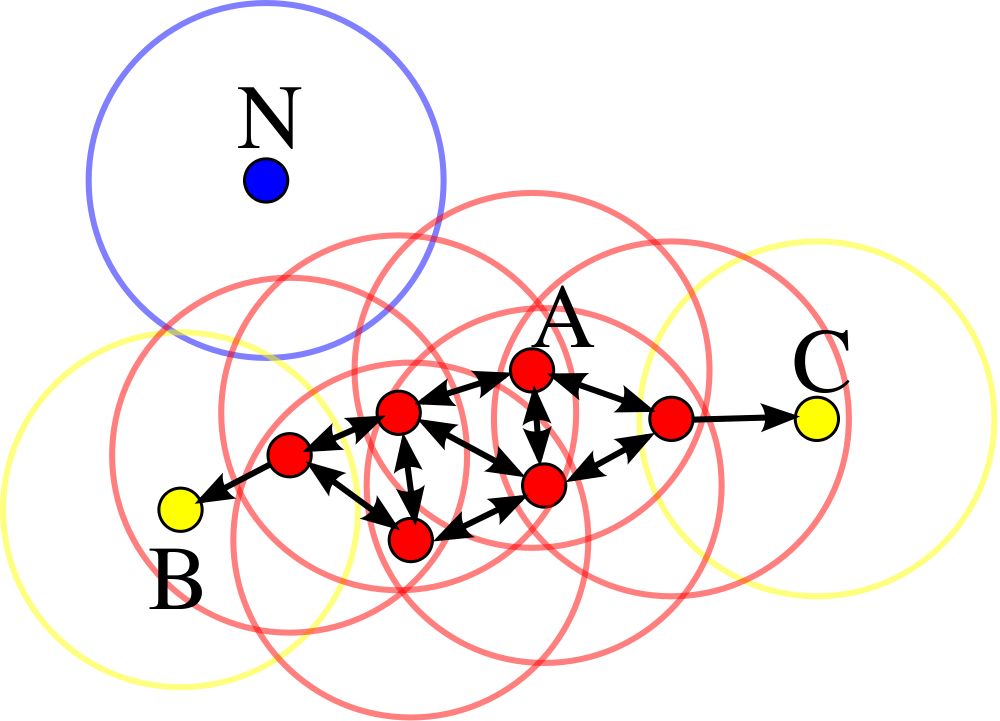
\includegraphics[width=0.8\textwidth]{images/DBSCAN-Illustration.png}
		\caption{Illustration of core points(red), border points(yellow), and outlier(blue)~\cite{wiki:DBSCAN}. In the illustration, $MinPts = 4$, $Eps$ is the radius of those circles.}
		\label{fig:DBSCANConcept}
	\end{center}
\end{figure}

As show in the figure, red points are core points since in each red circle, there are at least 4 points(including the center point). While for the yellow point, they don't have enough points in their circles, but they embed in one of the red circles. Thus, they are border points. As for the blue point, it has neither enough point in the blue circle nor is in any red circle. Thus, the blue point an outlier/noise.

These definitions reveal the assumption and theory of DBSCAN. DBSCAN assumes that, each cluster consists of two types of points, core points and border points. Core points form inner denser areas compared to spaces outside of clusters. Border points form a slightly sparser areas surrounding the inner core areas, but still the density is higher than spaces between different clusters, possessed by noise. In DBSCAN, the density of an area is measured by the number of points centred at $u$ within an area specified by the given radius $Eps$. If there are at least $MinPts$ points, this area is considered to be a dense area. Thus, this area is part of a cluster. In the procedure \proc{Expand-Cluster}, the algorithm will explore the whole dense area and less dense border area belonging to the same cluster. Each call of \proc{Expand-Cluster} visits a different cluster. Thus, when the whole procedure \proc{DBSCAN} finishes, different clusters are formed.

\subsection{Analysis of DBSCAN}
\label{subsec:DBSCANalgorithm}
DBSCAN applies to a broader range of problems compared to K-Means. In K-Means, one of the obstacle is to compute the mean value. DBSCAN doesn't have this problem as long as the distance between points is computable. This enables DBSCAN to use more complicated distance measurement, such as edit distance, which is very useful in dealing with strings. Another advantage of DBSCAN is its robustness to noises. As mentioned in section~\ref{subsec:KMeansIssues}, the mean value will be heavily interfere by noises/outliers. In contrast, DBSCAN has a notion noises and it is able to spot these outliers, which is a core problem of this thesis. Finally, the most important advantage of DBSCAN is that it can find arbitrarily shaped clusters. It can even separate a cluster completely surrounded by a different cluster. An example is shown in Fig~\ref{fig:KMeansDBSCAN}.

\begin{figure}
	\begin{center}
		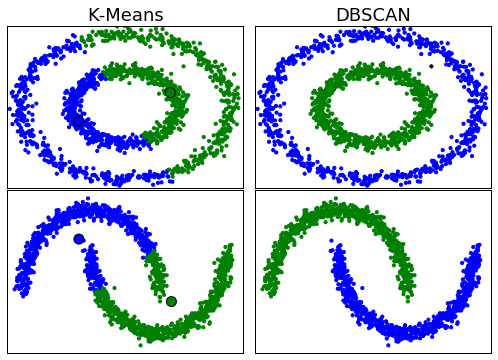
\includegraphics[width=\textwidth]{images/KMeansDBSCAN.png}
		\caption{A Comparison of K-Means and DBSCAN. In the diagram, two datasets ``circles'' and ``moons'' are used. Compared to K-Means, DBSCAN gives more reasonable clustering results on these two irregular shaped datasets.}
		\label{fig:KMeansDBSCAN}
	\end{center}
\end{figure}

Similar to K-Means, DBSCAN also requires user specified parameters. To get the optimal result, a careful choice of these parameters is needed. Finding the appropriate parameter can be achieved in the similar way by finding the elbow point as mentioned in section~\ref{subsec:KMeansIssues}. The user can pick a number for $MinPts$ first. Then, for each point, the distance from its $kth$ nearest neighbour is computed. After sorting these distances in descending order and plot them, a graph called \id{sorted k-dist graph} can be obtained. This graph reveals insights about the density distribution of the whole dataset reflected in how the \id{k-dist} varies. Then the $Eps$ can be set to the value corresponding to the elbow point. This heuristic works well as the graph won't differ too much for $k > 4$. An illustration of this approach is shown in Figure~\ref{fig:DBSCANParameter}.~\cite{ester1996density}

\begin{figure}
	\begin{center}
		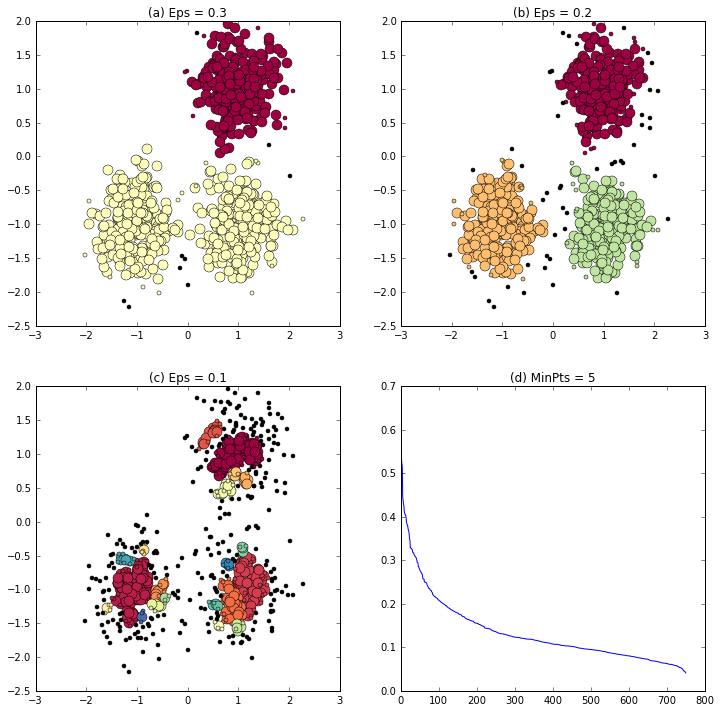
\includegraphics[width=\textwidth]{images/DBSCANParameter.png}
		\caption{Illustration of the heuristic parameter choosing approach for DBSCAN. (a)-(c) illustrates clustering results obtained by using different $Eps$. Each cluster is painted with a different color. Core points are represented using larger circles while border points are represented using smaller circles. Black small circles represent outliers. In figure (a), very few points are labelled as noise and the bottom two clusters are not distinguished. In figure (b), the result is more reasonable and can be considered as optimal. In figure (c), too many points are labelled as noise and more than 3 clusters are reported. According to the \id{k-dist graph} shown in (d), 0.2 should be the best value for $Eps$, which corresponds to the result in figure (b).}
		\label{fig:DBSCANParameter}
	\end{center}
\end{figure}